\documentclass[border=2pt]{standalone}
\usepackage{tikz}
\usetikzlibrary{through}
\usetikzlibrary{calc}
\usetikzlibrary{intersections}
\usetikzlibrary{backgrounds}


\begin{document}
    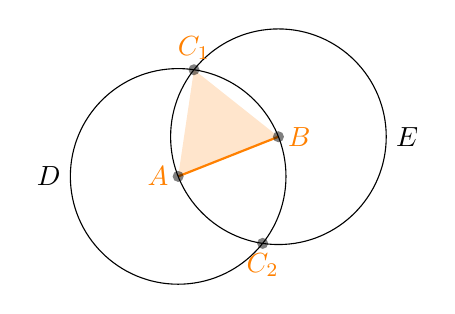
\begin{tikzpicture}
        \coordinate [label=left:$\textcolor{orange}{A}$] (A) at ($(0, 0)+0.1*(rand, rand)$);
        \coordinate [label=right:$\textcolor{orange}{B}$] (B) at ($(1.25, 0.5)+0.1*(rand, rand)$);
        \draw [orange, thick] (A) -- (B);

        \node (D) [draw, circle through=(B), label=left:$D$, name path=D] at (A) {};
        \node (E) [draw, circle through=(A), label=right:$E$, name path=E] at (B) {};

        \path [name intersections={of=D and E, by={
            [label=above:$\textcolor{orange}{C_1}$]C1,
            [label=below:$\textcolor{orange}{C_2}$]C2
        }}];
        
        \foreach \point in {A, B, C1, C2}
            \fill [black, opacity=0.5] (\point) circle (2pt);

        \begin{pgfonlayer}{background}
            \fill[orange!20!white] (A) -- (C1) -- (B) -- cycle;
        \end{pgfonlayer}
    \end{tikzpicture}
\end{document}